\chapter{Orbit Geometry}

%\epigraph{\textit{"Our two greatest problems are gravity and paperwork. We can lick gravity, but sometimes the paperwork is overwhelming."}}{Werner von Braun, 1958}

%\section{Introduction}
\section*{}
\paragraph{}
Throughout this chapter, the bases of orbital geometry will be explained in order to correctly understand the parameters that will later be exposed when dealing with the constellation orbits (or the position of the satellites in them). However, long theoretical explanations will be avoided so as not to distract the reader from the main objective of the project.

To understand the movement in space is enough to apply the Newton's laws. These, however, need an inertial non-rotating frame to be correctly described. When dealing with Earth-orbiting, one usually chooses a reference system called \textit{geocentric-equatorial system} which is shown in the figure~\ref{fig:eqframe} As can be seen, the XY plane coincides with the plane Equatorial with the X axis pointing in the direction of the vernal equinox \footnote{an imaginary line found by drawing a line from the Earth to the Sun on the first day of spring}. The Z axis correspond the axis of rotation of the earth and points to the north (following the right-hand rule).

\begin{figure}[H]
\centering
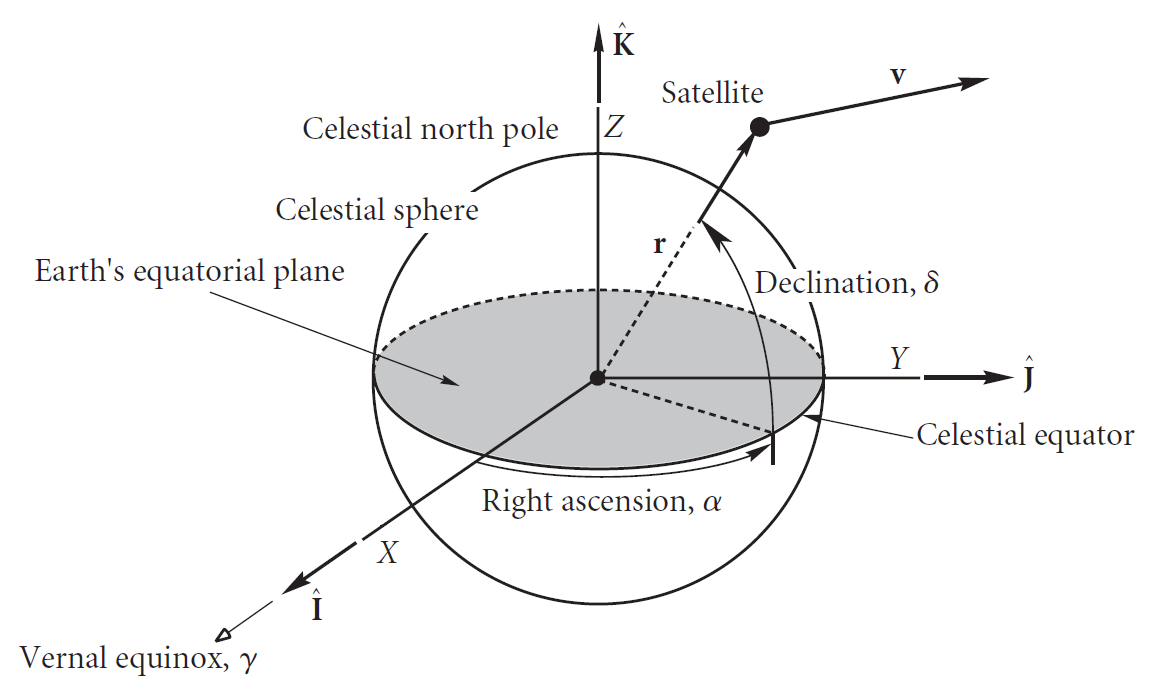
\includegraphics[scale=.55]{./Geometry/fig-Ch1-Geometry/eqframe.png}
\caption{Geocentric-equatorial frame. Extracted from \cite{Curtis2010}}
\label{fig:eqframe}
\end{figure}

By defining this system, any point in the space can be depicted by its position vector $r$ and we can study its movement by the velocity vector $\dot{r}$. These elements are useful especially for computational work but they nearly do not provide information about the orbit. For these reason, the orbital elements were developed.

\section{Keplerian Geometry}
\paragraph{}
The \textit{Classical Orbital elements}, also known as the \textit{Keplerian elements} as an attribution to Johannes Kepler, are six independent quantities which re sufficient to describe the size, shape and orientation of an orbit. This set of elements are shown in the figure~\ref{fig:COE} and are defined as follows:
\begin{itemize}
\item\textbf{Semi-major axis} ($a$): It is related to the size of the orbit and its defined by the sum of the apogee (furthest point) and the perigee (closest point) divided by two.
\item\textbf{Eccentricity} ($e$): It defines the shape of the orbit with respect to that of a circle. Thus, the eccentricity of a circular orbit is null while hyperbolic orbits have an eccentricity greater than one.
\begin{table}[H]
\centering
\label{tb:evalues}
\begin{tabular}{|l|c|}
\hline
Circular     & $e=1$   \\ \hline
Elliptical   & $0<e<1$ \\ \hline
Parabolic  	 & $e=1$   \\ \hline
Hyperbolic   & $e>1$   \\ \hline
\end{tabular}
\caption{Eccentricity values depending on the shape of the orbit}
\end{table}
\item\textbf{Inclination} ($i$): the inclination is the angle between the positive Z axis and the angular momentum vector ($\textbf{h}$) which is perpendicular to the orbital plane. The inclination of the orbit can take a value from $0\deg$ to $180\deg$. For $0\deg\leq i\leq 90\deg$ the motion \textit{posigrade} and for $90\deg\leq i\leq 180\deg$ the motion is \textit{retrogade}.
\item\textbf{Right ascension of the ascending node - RAAN} ($\Omega$): This parameter, along with the inclination define the orientation of the orbital plane. It is the angle between the positive X axis and the intersection of the orbital plane with the equatorial plane XY in counterclockwise direction. The intersection mentioned is called the node line and the point where the orbit passes through the node line (from south to north) is the ascension node ($0\deg\leq \Omega\leq 360\deg$).
\item\textbf{Argument of perigee} ($\omega$): Is defined as the angle between the ascending node and the perigee. It describes the orientation of the ellipse with respect to the frame ($0\deg\leq \omega\leq 360\deg$). 
\item\textbf{True Anomaly} ($\phi$): This last quantity is used to describe the satellite's instantaneous position with respect to the perigee. Is the angle, measured clockwise, between the perigee and the satellite position. From all the orbital elements, the true anomaly is the only that changes continuously. Sometimes, true anomaly is substituted by the mean anomaly, which can be calculated using another auxiliary angle called the eccentric anomaly.
\begin{equation}
\begin{gathered}
\cos E=\frac{e+\cos \theta}{1+e\cos \theta}\\
M=E-e\sin E
\end{gathered}
\end{equation}

\end{itemize}

\begin{figure}[H]
\centering
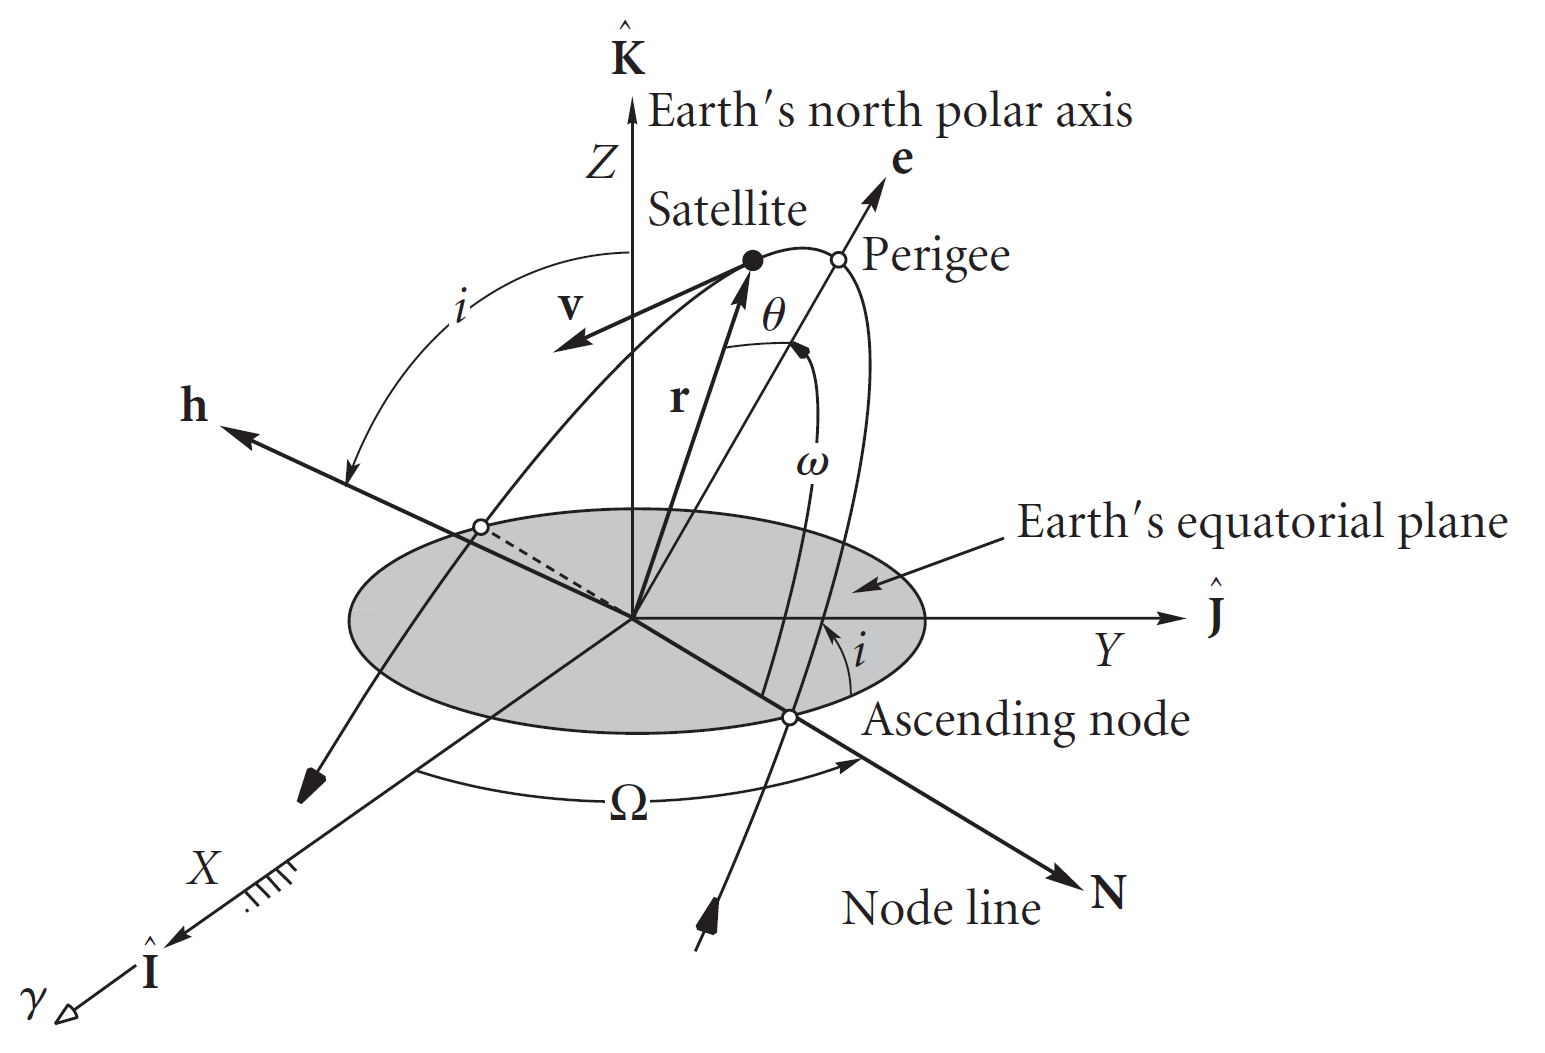
\includegraphics[scale=.3]{./Geometry/fig-Ch1-Geometry/COE.png}
\caption{Geocentric-equatorial frame and the Classical Orbital Elements. Extracted from \cite{Curtis2010}}
\label{fig:COE}
\end{figure}

\section{Dynamic equations}
\paragraph{}
As aforementioned, the motion of an object in the space can be described using the Newton's laws. The basic idea developed by Newton is to study the Cubesat and the Earth as a spherical bodies in mutual gravitational attraction and neglect the gravitational forces caused by other objects (this is called the \textit{two body} problem). The forces balance is simple since we only have the Earth gravitational attraction, which must compensate the centripetal acceleration of the satellite. Thus, using the law of universal gravitation,

\begin{equation}
-G\frac{M_{E}m_{sat}}{r^3}\vec{r}=m_{sat}\vec{a}_{sat}
\end{equation}

Where $G$ is the gravitational constant and $r$ represents the distance between the satellite and the Earth. From the last equation, we only want to obtain the acceleration, therefore:

\begin{equation}
-G\frac{M_{E}}{r^3}\vec{r}=\vec{a}_{sat}=\frac{d^2 \vec{r}}{d t^2}
\end{equation}

For simplicity, it usual to denote $\mu=GM_{earth}$ resulting in the following equation:

\begin{equation}\label{eq:a1}
-\frac{\mu}{r^3}\vec{r}=\frac{d^2 \vec{r}}{d t^2}
\end{equation}

This expression is a second order equation that models the motion of the Cubesat relative to the Earth and it can be analytically solved. The only problem is that several hypotheses have been applied that make the case different from reality. The formulation should be modified to take into account the effects due to:
\begin{itemize}
	\item More bodies attracting the satellite (Sun, Moon, Venus, etc.)
	\item The existence of more forces like the drag, the solar radiation pressure, etc.
	\item The earth is not an spherical body.
\end{itemize}
The corrections for considering these things are called perturbations and they are explained in the Chapter~\ref{ch:Pert} of this part of the report.
	